\begin{figure}[htbp]
\centering
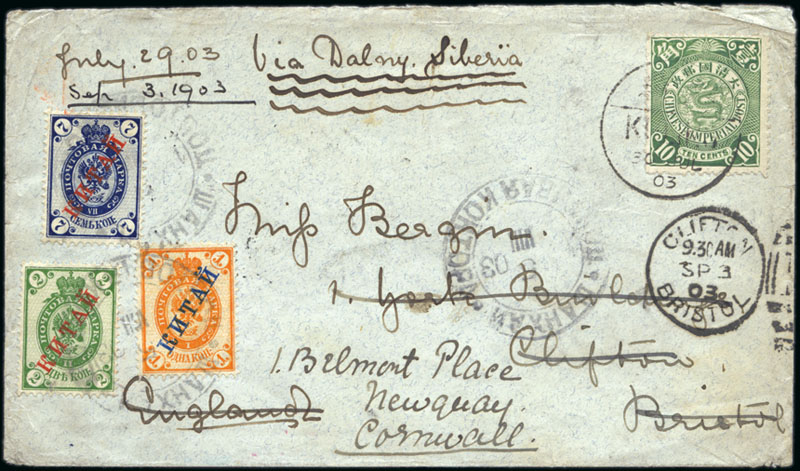
\includegraphics[width=.95\textwidth]{../russian-post-offices-in-china/10060.jpg}
\caption{
10060	SHANGHAI: 1903 Cover sent from KULING to England endorsed 
"via Dalny. Siberia," franked with China 10c Dragon tied by Kuling 
30.07.03 cds, sent via Kiukiang and Shanghai, where it was passed to 
the Russian P.O. and franked with "KITAI" 1k, 2k and 7k tied by Shanghai 
5.8.03 (Tchilinghirian type 1, Gregorian calendar), sent overland via 
Chinese Eastern and Trans-Siberian railways, with Moscow, Bristol, 
Clifton and Newquay transits.
\euro 1,800.00 
}  
\end{figure} 

\begin{figure}[htbp]
\centering
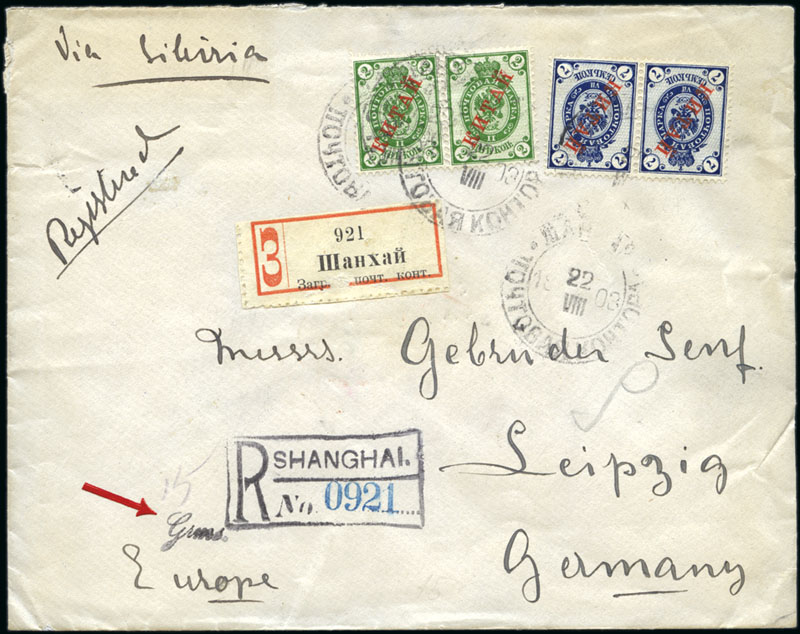
\includegraphics[width=.95\textwidth]{../russian-post-offices-in-china/10061.jpg}
\caption{
10061	SHANGHAI: 1903 Cover registered to Germany with pairs of "KITAI" 2k and 
7k tied by Shanghai 22.8.03 cds (T\&S type 1), with boxed registration hs in 
English and reg'd label in Cyrillic, Moscow bs, underpaid 2k but no tax mark, 
weight recorded (15 grams)
Note: A registration notice in a Western language was required by UPU regulations
\euro500.00.
}  
\end{figure} 

\begin{figure}[htbp]
\centering
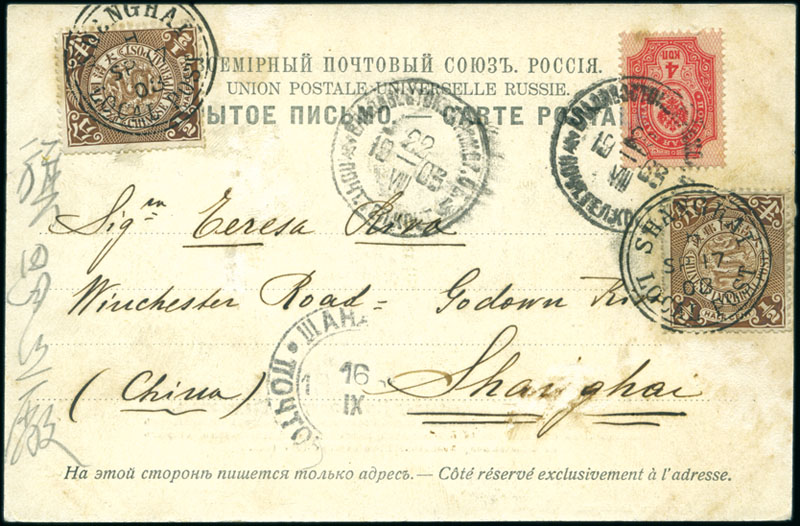
\includegraphics[width=.95\textwidth]{../russian-post-offices-in-china/10062.jpg}
\caption{
10062	SHANGHAI: 1903 Postcard from Vladivostok to Shanghai franked with Arms 
4k paying the UPU rate, with Russian P.O. Shanghai arrival (T\&S type 1, Gregorian 
calendar), passed to the Chinese P.O. and franked with two China 1/2c Dragons 
tied by "SHANGHAI / LOCAL POST," the imposition of a local delivery charge 
is very unusual.

Note: This was a time of tension between Russia and China owing to the 
continued presence of Russian troops in Manchuria.
\euro 300.00 
}  
\end{figure} 

\begin{figure}[htbp]
\centering
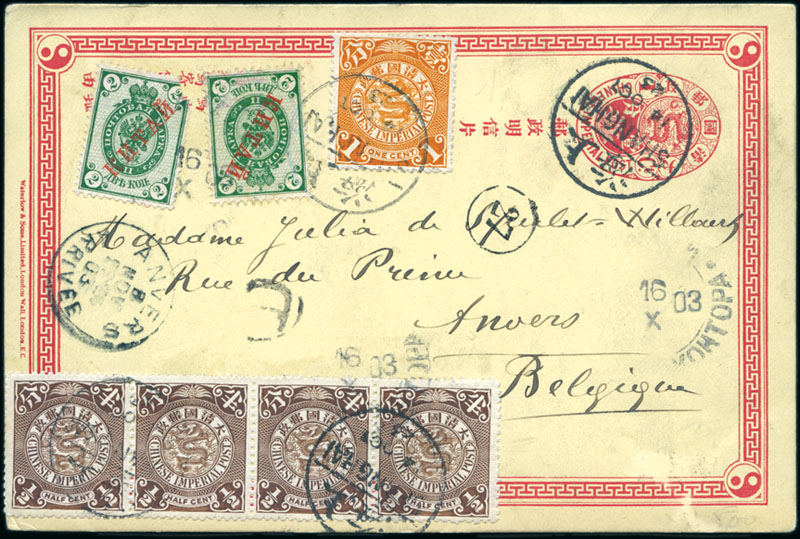
\includegraphics[width=.95\textwidth]{../russian-post-offices-in-china/10063.jpg}
\caption{
10063	SHANGHAI: 1903 China 1c postcard to Belgium uprated with 1/2c 
strip of four and 1c Dragons, tied by Shanghai bilingual 14.10.03 cds, 
transferred to the Russian P.O. where two "KITAI" 2c were applied 
(corner defect on one) and tied by Shanghai cds (T\&S type 1), Anvers arrival, 
a fine and attractive mixed country combination.
Note: China was not a member of the UPU at this time so stamps of one of 
the foreign post offices was needed to convey mail abroad.
\euro 400.00. 
}  
\end{figure} 

\begin{figure}[htbp]
\centering
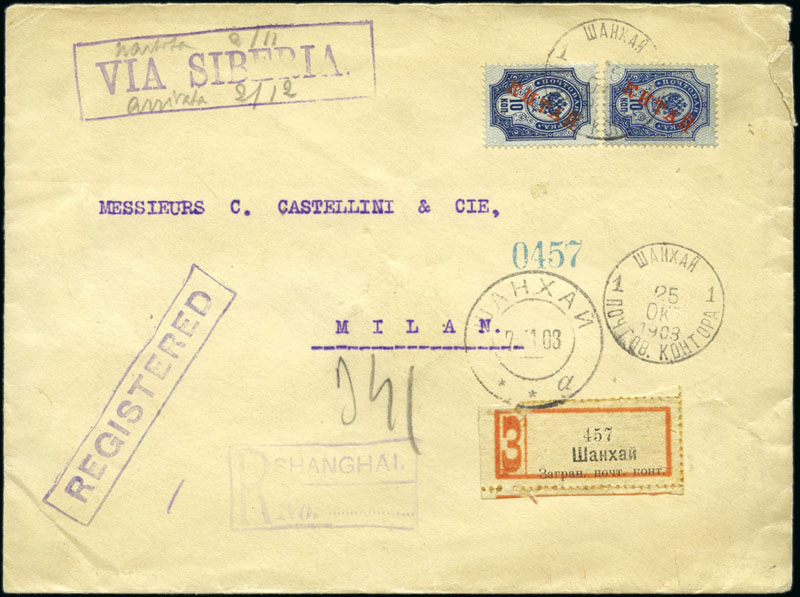
\includegraphics[width=.95\textwidth]{../russian-post-offices-in-china/10064.jpg}
\caption{
10064		ZoomSHANGHAI: 1903 Cover sent registered to Italy with two "KITAI" 
10k tied by Shanghai 25.10.03 cds (T\&S type 2, Julian calendar) with further 
cds adjacent (T\&S type 3, Gregorian calendar), with boxed registration hs in 
English and label in Cyrillic, a scarce usage of the type 2 cds as a cancel 
which was mainly used for transit and arrival markings, routed overland to 
take advantage of newly opened Tran-Siberian Railway
\euro 300.00 
}  
\end{figure} 

\begin{figure}[htbp]
\centering
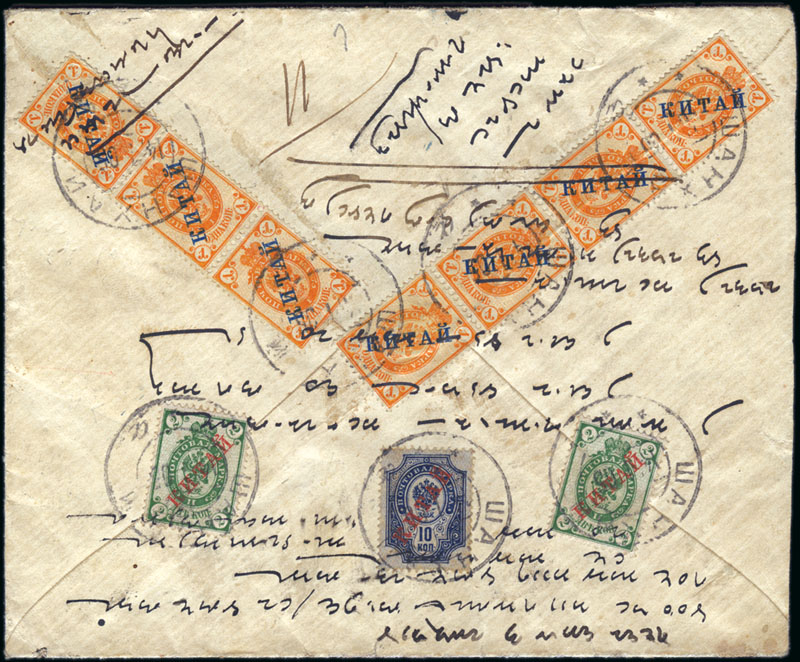
\includegraphics[width=.95\textwidth]{../russian-post-offices-in-china/10065.jpg}
\caption{
10065 SHANGHAI: 1905 Cover addressed in Farsi, Russian and English, 
sent registered to Bukhara (in modern day Uzbekistan) franked on the reverse 
with "KITAI" 1k (7, all used to seal the envelope), 2k (2) and 10k tied by 
Shanghai 14.1.05 cds (T\&S type 3), registered label on obverse, unusual

\euro 500.00 
}  
\end{figure} 



                                                                              